\autsubsection{Ice temperature profile}{Kristian Sloth Lauszus}
\label{sec:IceTemperatureProfile}

%* Indirect: salinity, melting speed
%* Drill sample
%* Passive screw in the tip
%	* Thermal isolated
%* Measure heat conductivity of the water
%	* Can be used to estimate the salinity of the water
%		* Melting speed
%
%* "back of the envelope" calculations

In order to estimate the descent time it is important to know the ice temperature profile i.e. the temperature change as a function of the depth and the energy required in order to melt the column of ice. The thermal conductivity of polycrystalline ice can be calculated according to the following equation\cite[(2.3)]{article:thermalConductivity}:
\begin{equation}
	k(T) = \frac{a_1}{T} + a_0
\end{equation}
Where the constants $a_1$ and $a_0$ are given by:
\begin{align}
	a_1 &= \unitfrac[4.88 \e7]{ergs}{cm \, s} \\ \nonumber
		&= \unitfrac[488]{W}{m} \\
	a_0 &= \unitfrac[4.68 \e4]{ergs}{cm \, K \, s} \\ \nonumber
		&= \unitfrac[0.468]{W}{m \, K}
\end{align}
The boundary conditions for the temperature is simply given by 273.15 K at the transition between the water and ice and 100 K at the surface of the moon\cite{article:thermalConductivity}. Thus the temperature difference can be calculated:
\begin{align}
	& T_m = \unit[273.15]{K} \\
	& T_s = \unit[100]{K} \\
	& T_\Delta = T_m - T_s = \unit[173.15]{K}
\end{align}
Figure \ref{fig:T_vs_k} shows two plots of the thermal conductivity as a function of the temperature. Figure \ref{fig:T_vs_k_full} shows the thermal conductivity from 0 K to 273.15 K, figure \ref{fig:T_vs_k_zoom} on the other hand shows only shows the thermal conductivity in the range of the boundary conditions.
\begin{figure}[htb]
	\centering
	\subfloat[From 0 K to 273.15 K]{
		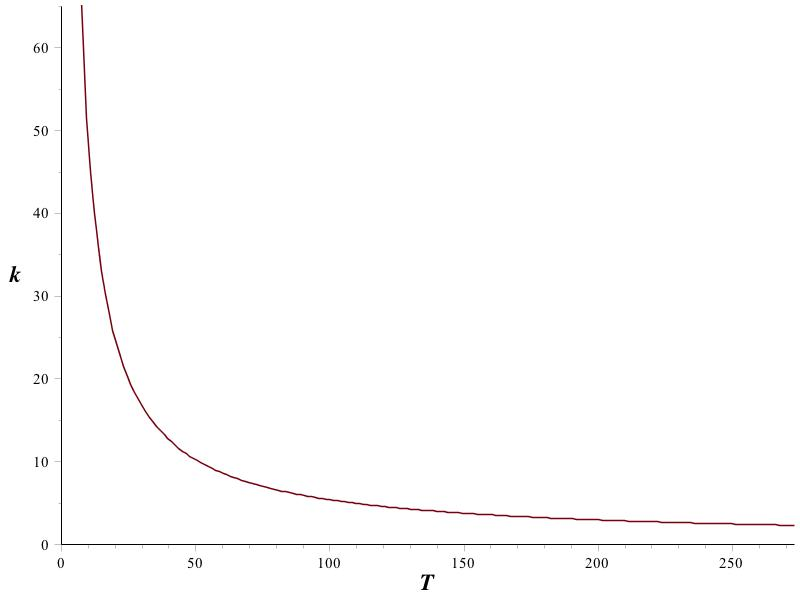
\includegraphics[width=.48\textwidth]{figures/temperature/T_vs_k}
		\label{fig:T_vs_k_full}
	}
	\subfloat[From $T_s$ to $T_m$]{
		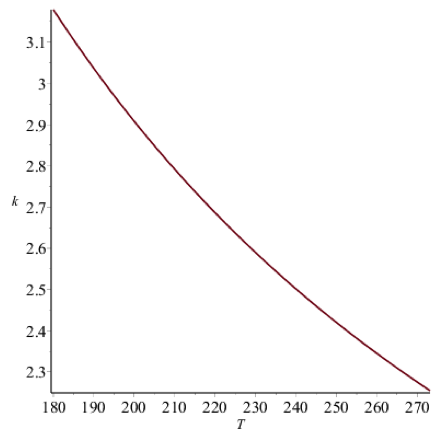
\includegraphics[width=.48\textwidth]{figures/temperature/T_vs_k_zoom}
		\label{fig:T_vs_k_zoom}
	}
	\caption{Thermal conductivity as a function of the temperature}
	\label{fig:T_vs_k}
\end{figure}
The conductive heat transfer can be calculated fairly easily using Fourier's Law\cite{website:conductiveHeatTransfer}:
\begin{align}
	q(T) &= \frac{k(T) A T_\Delta}{d}
\end{align}
The area $A$ is the area of the penetrator facing the ice and by assuming a cylinder with a radius of 10 cm the area is given by:
\begin{align}
	A &= \pi \, 0.1^2 \approx \unit[0.03]{m^2}
\end{align}
Figure \ref{fig:T_vs_q} shows a plot of the conductive heat transfer as a function of the temperature. The thickness of the ice $d$ is assumed to be 3 km according to chapter \ref{sec:structural_profile}.
\begin{figure}[htb]
	\centering
	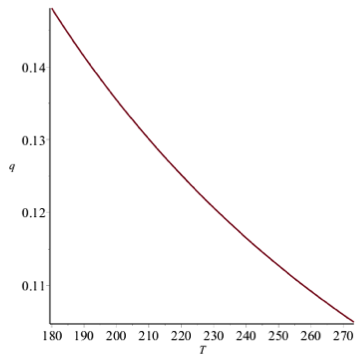
\includegraphics[width=.48\textwidth]{figures/temperature/T_vs_q}
	\caption{Conductive heat transfer as a function of the temperature}
	\label{fig:T_vs_q}
\end{figure}
Notice how both the conductive heat transfer $q$ and the thermal conductivity $k$ are approximately constant doing the interval $T_s$ to $T_m$, thus they can both be approximated by the average over the interval:
\begin{align}
	\bar{k} &= \unitfrac[3.80]{W}{m \, K} \\
	\bar{q} &= \unit[0.0066]{W}
\end{align}
Now the temperature as a function of the depth $d$ can be calculated assuming that the heat transfer and thermal conductivity are constant throughout the ice:
\begin{align}\label{eq:T_d}
	T(d) &= T_s + d \frac{\bar{q}}{\bar{k} A} = 100 K + \unitfrac[0.058 d]{K}{m}
\end{align}
Figure \ref{fig:d_vs_T} shows a plot of the temperature as a function of the depth into the ice.
\begin{figure}[htb]
	\centering
	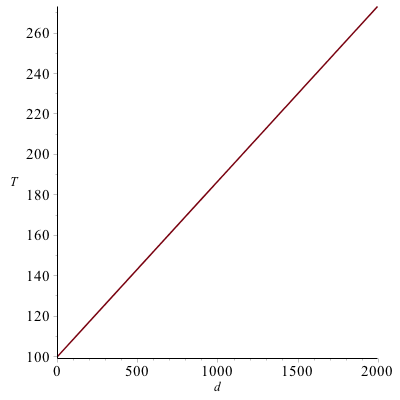
\includegraphics[width=.48\textwidth]{figures/temperature/d_vs_T}
	\caption{Temperature as a function of the depth}
	\label{fig:d_vs_T}
\end{figure}
Figure \ref{fig:T_vs_rho} shows the density of ice as a function of the temperature using the values found in Table \ref{tab:ice_density}. This is be approximated by a linear second order function:
\begin{equation}\label{eq:rho_approx}
	\rho(T) = 931.21 - 0.68 \e{-3} T - 0.19 \e{-3} T^2
\end{equation}
Figure \ref{fig:T_vs_rho_approx} shows a plot of the approximated density of ice as a function of the temperature.
\begin{figure}[htb]
	\centering
	\subfloat[Density of ice according to Table \ref{tab:ice_density}]{
		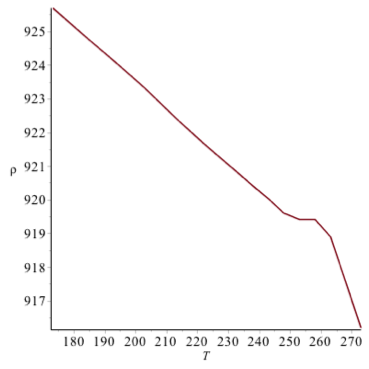
\includegraphics[width=.48\textwidth]{figures/temperature/T_vs_rho}
		\label{fig:T_vs_rho}
	}
	\subfloat[Approximated ice density using \eqref{eq:rho_approx}]{
		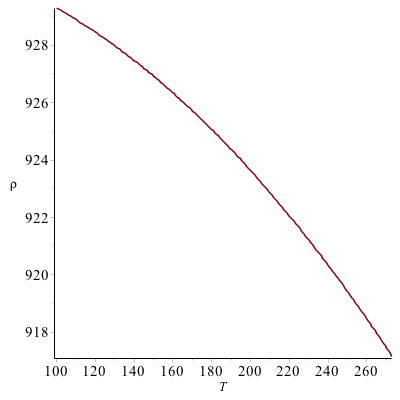
\includegraphics[width=.48\textwidth]{figures/temperature/T_vs_rho_approx}
		\label{fig:T_vs_rho_approx}
	}
	\caption{Density of ice as a function of the temperature}
\end{figure}
\begin{table}[htb]
	\centering
	\resizebox{\textwidth}{!}{%
	\begin{tabular}{|c|c|c|c|c|c|c|c|c|c|c|c|c|c|c|c|}\hline
		$\mathbf{T} ~ (K)$ & 273.15 & 268.15 & 263.15 & 258.15 & 253.15 & 248.15 & 243.15 & 238.15 & 233.15 & 223.15 & 213.15 & 203.15 & 193.15 & 183.15 & 173.15 \\ \hline
		$\mathbf{\rho} ~ (\unitfrac{kg}{m^3})$ & 916.2 & 917.5 & 918.9 & 919.4 & 919.4 & 919.6 & 920.0 & 920.4 & 920.8 & 921.6 & 922.4 & 923.3 & 924.1 & 924.9 & 925.7 \\ \hline
	\end{tabular}}
	\caption{Density of ice for different temperatures\cite{website:iceDensity}}
	\label{tab:ice_density}
\end{table}
Now the density as a function of the distance can be calculated by inserting \eqref{eq:T_d} into \eqref{eq:rho_approx}:
\begin{equation}\label{eq:rho_approx_d}
	\rho(d) = 929.29 - 0.22 \e{-2} d - 6.19 \e{-7} d^2
\end{equation}
%A plot of \eqref{eq:rho_approx_d} and \eqref{eq:T_diff} can be seen in Figure \ref{fig:d_vs_rho} and Figure \ref{fig:d_vs_T_delta} respectively.
%\begin{figure}[htb]
%	\centering
%	\captionsetup[subfigure]{width=0.45\textwidth}
%	\subfloat[Ice density as a function of the depth using \eqref{eq:rho_approx_d}]{
%		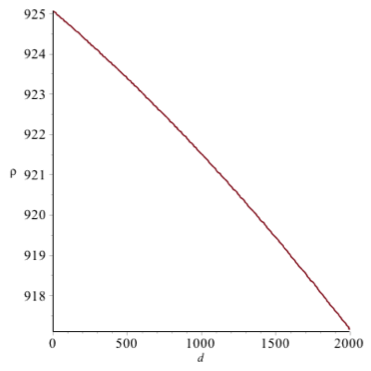
\includegraphics[width=.48\textwidth]{figures/temperature/d_vs_rho}
%		\label{fig:d_vs_rho}
%	}
%	\subfloat[Temperature difference as a function of the depth]{
%		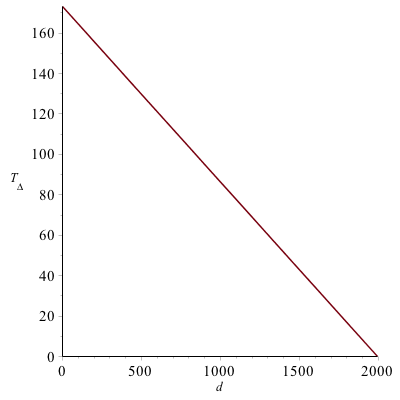
\includegraphics[width=.48\textwidth]{figures/temperature/d_vs_T_delta}
%		\label{fig:d_vs_T_delta}
%	}
%	\caption{}
%\end{figure}
Figure \ref{fig:T_vs_Cice} shows the specific heat capacity of ice plotted using the data found in Table \ref{tab:ice_heat_capacity}. Again this is approximated using a linear second order function:
\begin{equation}\label{eq:Cice_approx}
	C_{ice}(T) = -372.95 + 12.34 T - 0.013 T^2
\end{equation}
The specific heat capacity of ice as a function of the distance can be calculated by inserting \eqref{eq:T_d} into \eqref{eq:Cice_approx}:
\begin{equation}\label{eq:Cice_approx_d}
	C_{ice}(d) = 734.76 + 0.57 d - 0.42 \e{-4} d^2
\end{equation}
A plot of the approximated specific heat capacity can be seen in Figure \ref{fig:T_vs_Cice_approx}.
\begin{figure}[htb]
	\centering
	\subfloat[Specific heat capacity of ice according to Table \ref{tab:ice_heat_capacity}]{
		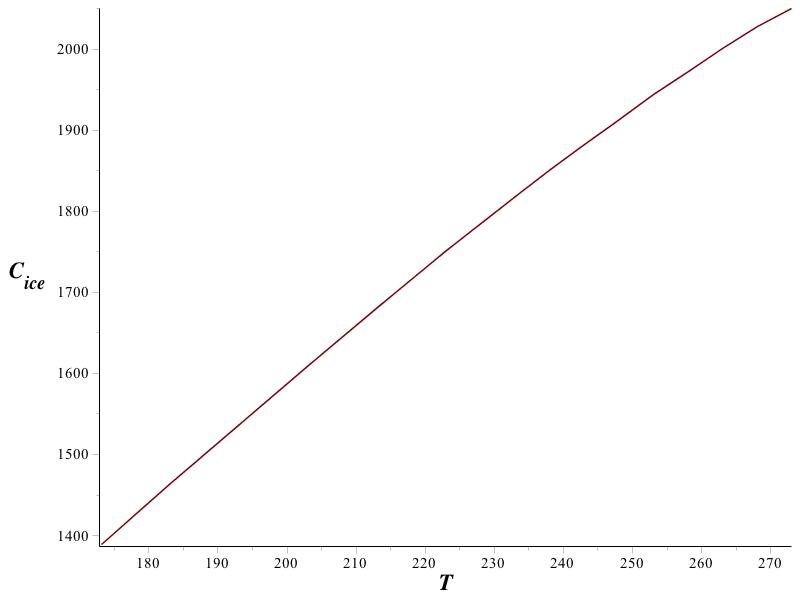
\includegraphics[width=.48\textwidth]{figures/temperature/T_vs_Cice}
		\label{fig:T_vs_Cice}
	}
	\subfloat[Approximated specific heat capacity of ice using \eqref{eq:Cice_approx}]{
		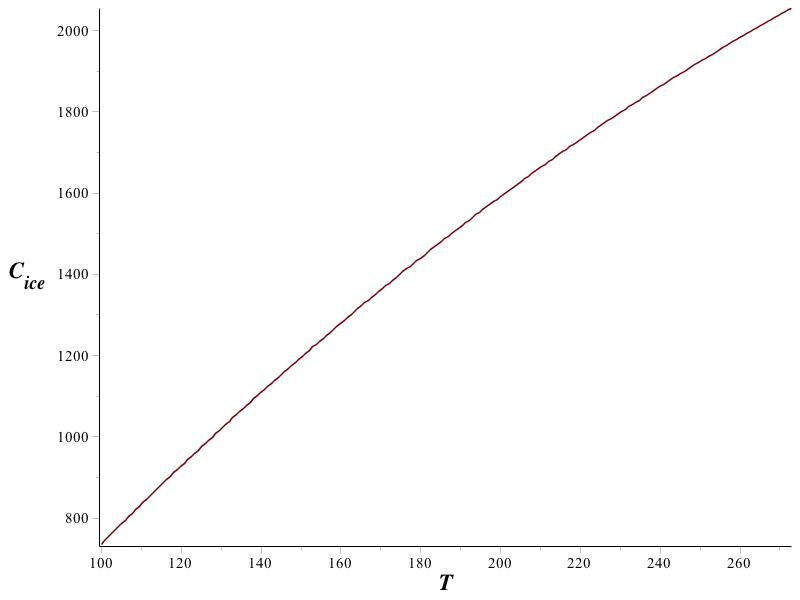
\includegraphics[width=.48\textwidth]{figures/temperature/T_vs_Cice_approx}
		\label{fig:T_vs_Cice_approx}
	}
	\caption{Specific heat capacity of ice as a function of the temperature}
\end{figure}
\begin{table}[htb]
	\centering
	\resizebox{\textwidth}{!}{%
	\begin{tabular}{|c|c|c|c|c|c|c|c|c|c|c|c|c|c|c|c|}\hline
		$\mathbf{T} ~ (K)$ & 273.15 & 268.15 & 263.15 & 258.15 & 253.15 & 248.15 & 243.15 & 238.15 & 233.15 & 223.15 & 213.15 & 203.15 & 193.15 & 183.15 & 173.15 \\ \hline
		$\mathbf{C_{ice}} ~ (\unitfrac{J}{K \, kg})$ & 2050 & 2027 & 2000 & 1972 & 1943 & 1913 & 1882 & 1851 & 1818 & 1751 & 1681 & 1609 & 1536 & 1463 & 1389 \\ \hline
	\end{tabular}}
	\caption{Specific heat capacity of ice for different temperatures\cite{website:iceDensity}}
	\label{tab:ice_heat_capacity}
\end{table}
%\begin{figure}[htb]
%	\centering
%	\includegraphics[width=.48\textwidth]{figures/temperature/d_vs_C_ice}
%	\caption{Specific heat capacity of the depth}
%	\label{fig:d_vs_C_ice}
%\end{figure}
The amount the temperature needs to be raised as a function of the distance is given by:
\begin{equation}\label{eq:T_diff}
	T_\Delta(d) = T_m - T(d) = 173.15 K - \unitfrac[0.058 d]{K}{m}
\end{equation}
The energy required to heat up the 3 km cylinder of ice to 0 \textdegree C can now be calculated:
\begin{align}
	E_0 &= A \, \int_0^{3\e{3}} \! C_{ice}(d) \, \rho(d) \, T_\Delta(d) \ \mathrm{d}d \\ \nonumber
	    &= \unit[8.93 \e{9}]{J}
\end{align}
The total mass of a 3 km cylinder of ice with an area of $A$ is given by:
\begin{equation}\label{eq:ice_total_mass}
	m_{total} = A \, \int_0^{3\e{3}} \! \rho(d) \ \mathrm{d}d = \unit[83174]{kg}
\end{equation}
Latent heat of melting of ice is given by\cite{website:waterLatentHeat}:
\begin{equation}
	L_m = \unitfrac[333.55 \e{3}]{J}{kg}
\end{equation}
The energy required for the phase change can now be calculated:
\begin{equation}
	E_{phase} = L_m m_{total} = \unit[2.77 \e{10}]{J}
\end{equation}
The total amount of energy is then given by:
\begin{equation}\label{eq:E_total}
	E_{total} = E_0 + E_{phase} = \unit[3.67 \e{10}]{J}
\end{equation}
It is noticeable that the energy required for the phase change takes up about 75 \% of the total energy, thus the approximations regarding the thermal conductivity, conductive heat transfer, and heat capacity should not have a huge impact on the result.

However the model of the ice density has a impact on the energy calculations of the phase change, as seen by \eqref{eq:ice_total_mass}. Thus a better model of the ice density would be beneficial. Further studies of the ice composition will be needed in this case, as the ice is assumed to be an isotropic and homogeneous material in the previous calculations. Furthermore the temperature at which the phase change occurs depends on the pressure as well.
% This will be discussed more in detail in chapter \ref{sec:temp_simulation}.
% Heat capacity and density is approximated below -100 C.

It is also noticeable that the energy required to melt the ice will be higher in practice than the total energy calculated in \eqref{eq:E_total}, as their will never be a 100 \% thermal energy transportation efficiency between the melting-device and the ice.

\subsubsection{Pressure Profile}

* What is the outside pressure?

\subsubsection{Simulation Results}\label{sec:temp_simulation}

\subsubsection{Simulation Validation}

* Should show that the "back of the envelope" calculations are right

\begin{figure}[htb]
	\centering
	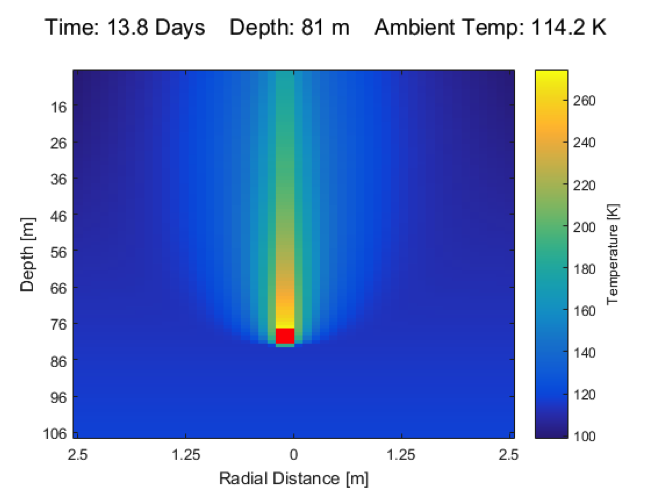
\includegraphics[width=\textwidth]{figures/temperature/temperature_simulation}
	\caption{TODO: Caption}
	\label{fig:temperature_simulation}
\end{figure}

\autsubsection{Water convection}{Kristian Sloth Lauszus and Lukas Christensen}

In this section the concept of natural convection will be presented and CFD (computational fluid dynamics) simulations will be used in order to estimate the natural convection for the penetrator.
\\
\\
Natural convection is interesting as it might be a means of transporting the water from the tip to inside the penetrator passively, guiding the water to the different instruments.  This is needed, as it would be interesting to analyse the salinity and various other elements in the melted water as the penetrator descents. The passive system would eliminate the needs for a pump system, which will add to the complexity and mass of the penetrator.

A sketch of the proposed water transportation system can be seen in Figure \ref{fig:water_transportation}. The intentions is to have the water flow from the intake to the end of the penetrator while running pass the different instruments placed in chambers along the exterior of the penetrator. The flute shape in the tip is intended to guide the water to the intakes in the side. This shape will also be useful in order to guide dirt, small rocks and other small items away from the front of the penetrator, which will improve the heat transfer efficiency between the tip and the ice. Furthermore the screw in the tip, as shown in Figure \ref{fig:water_transportation}, can be used for direct measurement of the temperature of the ice. However it will be important to thermally isolate this from the melter and/or compensate for its effect on the temperature measurement, so the true temperature of the ice can be obtained. Another option would be to have an active screw going into the ice a certain intervals, but the passive system is desirable due to simplicity of this design. % TODO: YouTube video
\begin{figure}[htb]
	\centering
	\captionsetup[subfigure]{width=0.25\textwidth}
	\subfloat[Sketch of the penetrator with flute shape used for dirt removal and water redirection]{
		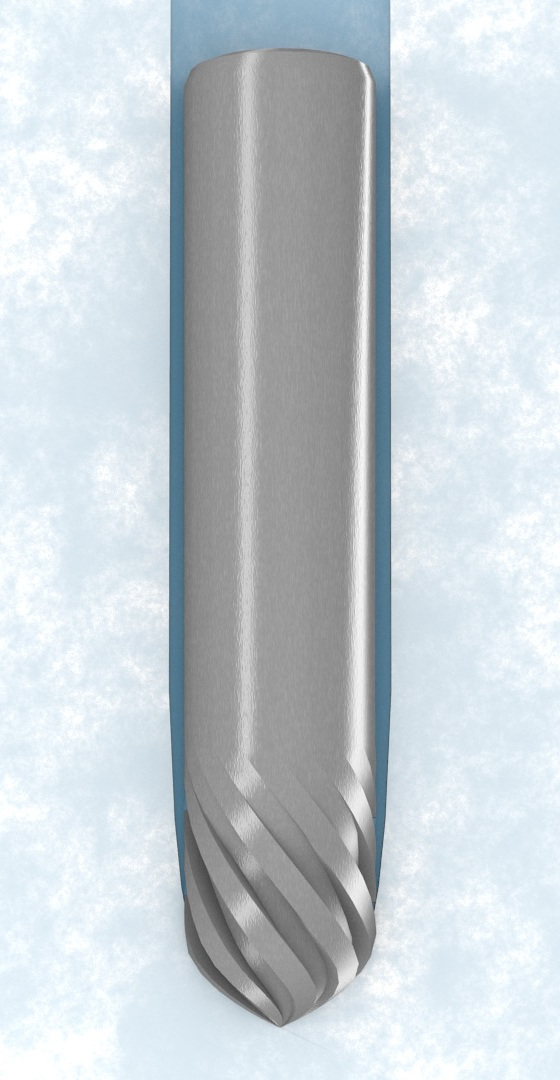
\includegraphics[width=.3\textwidth]{figures/convection/penetrator_model_cropped}
		\label{fig:penetrator_model}
	}
	\subfloat[Cross-section showing the passive water transportation system]{
		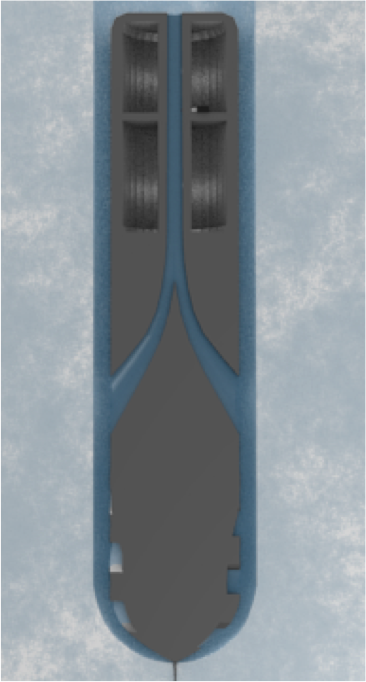
\includegraphics[width=.3\textwidth]{figures/convection/water_transportation}
		\label{fig:water_transportation}
	}
	\caption{Sketch of the penetrator design}
%	\label{fig:}
\end{figure}
\\
Natural convection is caused by density gradients due to temperature differences in a fluid. In this example the water near the tip will be warmer than the water located at behind the penetrator this will cause the less dense water in the bottom to rise with a certain velocity, thus we can take advantage of this effect and redirect the water from the tip to the inside of the penetrator, as explained earlier\cite{website:naturalConvectionPdf}.

An important number associated with natural convection is the so-called Rayleigh number $\mathbf{Ra}$, which is given by\cite{website:naturalConvectionWiki}:
\begin{equation}
	\mathbf{Ra} = \frac{\Delta\rho g L^3}{\alpha \mu}
\end{equation}
If the Rayleigh number is larger than a certain critical value, natural convection occurs. $\Delta\rho$ is the difference in density. It can be approximated using the temperature at the bottom and top of the penetrator and then inserting them into \eqref{eq:rho_approx}. $g$ is the local gravitational acceleration. In this case it is 0.134 g on Europa\cite{website:europaGravity}. $L$ is the characteristic length and can be approximated as the length of the penetrator. This is only an approximation as the water column above will also effect the convection. $\alpha$ and $\mu$ are the thermal diffusivity and dynamic viscosity of the fluid. % Note that the length of the penetrator will have a huge impact on the water flow, as the the Rayleigh number is proportional to the characteristic length third, thus the natural convection can be increased a lot by increasing the length of the penetrator.

% TODO:
	% How to measure melting speed
	% Measure heat conductivity of the water
		% Can be used to estimate salinity - can perhaps be used to estimate the melting speed?

\subsubsection{CFD analysis}
In an effort to evaluate the feasibility of passive thermal convection a CFD (Computational Fluid Dynamics) analysis has been performed. The software Autodesk CFD was utilized for this purpose. 
\\
\\
Figure \ref{fig:3d_model} shows a CAD model of a potential penetrator design. The model was simplified to have a channels having the same effect as the flutes resulting in guiding the water into the intakes and further inside the penetrator. However, due to the complexity a even simpler model was made, as shows in Figure \ref{fig:simplified_3d_model}. 
\begin{figure}[htb]
	\centering
	\subfloat{
		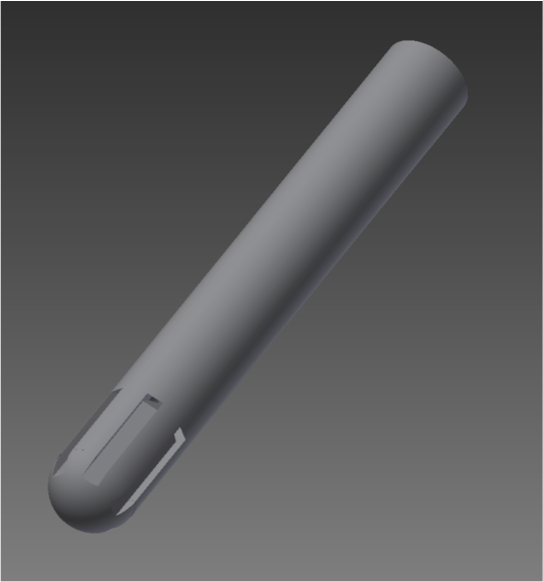
\includegraphics[width=.48\textwidth]{figures/convection/3d_model}
	}\\
	\subfloat{
		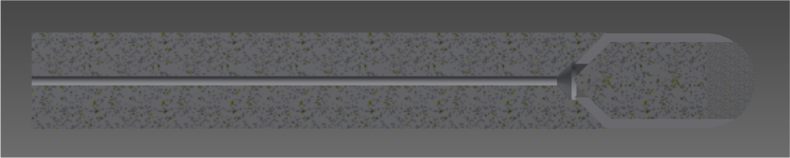
\includegraphics[width=.48\textwidth]{figures/convection/3d_model_inside}
	}
	\caption{3D model of the penetrator design}
	\label{fig:3d_model}
\end{figure}
\\
The simplified model is made of a totally separated heating element in the front of a hollow cylinder. This means that heat will not be conducted from the heater into the bulk of the penetrator. While this is not very realistic, it provides the best possible scenario for convection as it leads to a very large temperature gradient along the length of the penetrator.
\begin{figure}[htb]
	\centering
	\subfloat[Simplified 3D model used for CFD analysis]{
		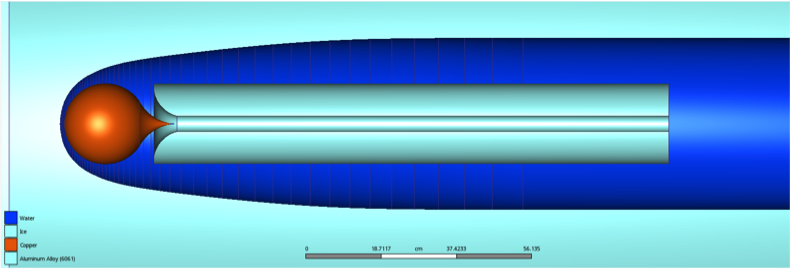
\includegraphics[width=.6\textwidth]{figures/convection/simplified_3d_model}
		\label{fig:simplified_3d_model}
	}\\
	\subfloat[CFD temperature simulation results]{
		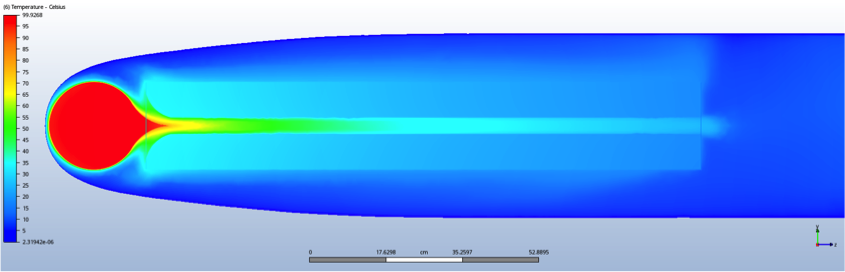
\includegraphics[width=.6\textwidth]{figures/convection/cfd_temperature}
	}\\
	\subfloat[CFD velocity simulation results]{
		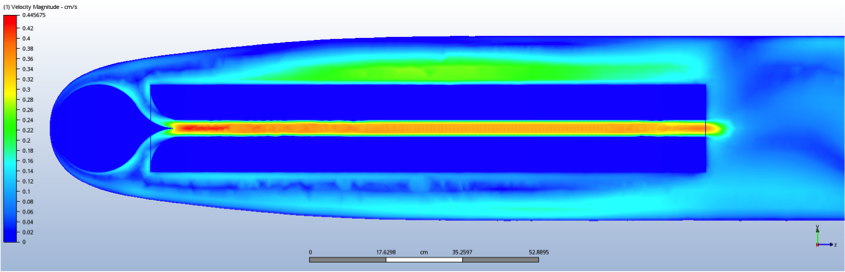
\includegraphics[width=.6\textwidth]{figures/convection/cfd_velocity}
	}
	\caption{CFD simulation results}
	\label{fig:cfd}
\end{figure}
\\
The ice that surrounds the penetrator was designed so as to mimic the expected shape of the bore hold with it being narrow at the heating element and then expanding out to a fixed width near the middle of the penetrator. The diameter of the bore hole is somewhat over exaggerated allowing flow around the penetrator, again, to ensure the best conditions possible for convection.
\\
\\
The internal diameter of the penetrator model is 4 cm, which was chosen because the much smaller diameters resulted in breakdown of the simulation. The heater is simulated as being made of solid copper with a 2000 W internal heat source, while the bulk of the penetrator is made of aluminum. The control volume represents some 4 m of water column with the top being designated as an open surface, meaning that the simulation allows flow through it, as if it was extended indefinitely. The pressure and ambient temperature was set to 120 bar and 0 $^\circ C$, respectively.
\\
\\
By using these boundaries conditions a steady-state CFD analysis was made the result of which is displayed in Figures \ref{fig:cfd} b and c. It should be noted that an adaptive mesh was used to ensure maximum detail within the penetrator.
It can be seen that the heating element reaches a temperature of around 100 \textdegree C and the back of the penetrator stabilizes near 15 \textdegree C. This results in a natural convection flow through the penetrator at only 0.4 cm/s or 200 s/L. Considering that this result was obtained using unrealistically good conditions and with no resistances inside the penetrator, like for example a filtering system. Thus, a pump system, such as a peristaltic pump, is properly needed to ensure proper water flow to the different instruments in the penetrator. This will be discussed more in detail in chapter \ref{sec:water_flow}.

% TODO: Comment on different assumptions
	% I følge simuleringen så bliver den cirka 100 grader (celsius). Reelt vil det nok være mindre, fordi varmen skal fordeles rundt i hele penetratoren
	% Cirka 10-15 grader, hvis vi følger CFD simuleringen, hvilket passer meget godt med smelte-simuleringen


